\documentclass{article}
\usepackage{siunitx} 
\usepackage{graphicx}
\usepackage{natbib}
\usepackage{amsmath} 

\setlength\parindent{0pt}

\renewcommand{\labelenumi}{\alph{enumi}.}

%\usepackage{times} 

%----------------------------------------------------------------------------------------
%	DOCUMENT INFORMATION
%----------------------------------------------------------------------------------------

\title{Práctica 12 \\ Programación Concurrente y de Tiempo Real \\Universidad de Cádiz} % Title

\author{Alejandro Serrano Fernández} % Author name

\date{\today} % Date for the report

\begin{document}

\maketitle % Insert the title, author and date


%----------------------------------------------------------------------------------------
%	SECTION 1
%----------------------------------------------------------------------------------------

\section{Ejercicio 1}
Para calcular el tiempo que tarda mi computadora en calcular el tiempo que tarda en realizar la convolución de una matriz de 1000 elementos, cabe destacar que los siguientes datos han sido obtenidos a través de un portátil equipado con un i7-7700hq de 4 núcleos y 8 threads. 

\hfill\break
Pues bien, sobre el sistema operativo Windows podemos observar que para tanto Java(azul) como C++(Naranja) se obtiene un menor tiempo cada vez que aumentamos el número de hilos, sin embargo, a partir de 8 threads observamos lo contrario. Destacar también, que para el mismo problema, obtenemos mejores resultados en C++ que en Java, esto puede ser debido a que Java hace uso de la máquina virtual para ejecutarse.


\begin{figure}[h]
\centering
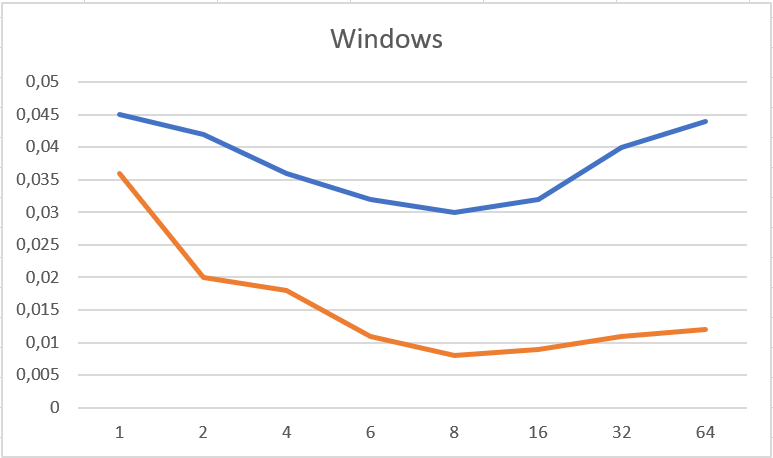
\includegraphics[scale=0.5]{windows.png}
\caption{Tiempos en Windows}
\end{figure}


\hfill\break
\begin{figure}[h]
\centering
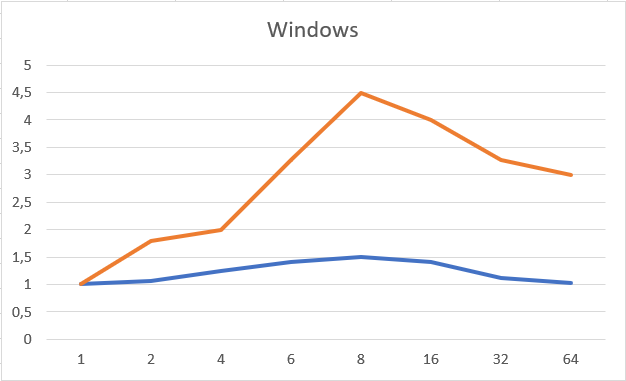
\includegraphics[scale=0.7]{speed-up windows.png}
\caption{SpeedUp en Windows}
\end{figure}

En cuento a Linux, observamos que obtenemos resultados similares a los obtenidos en Windows, aunque ligeramente algo inferiores, pues hay un ligero aumento de tiempo en comparación con Windows. En ambos sistemas operativos, a partir de 8 núcleos comienza a subir ligeramente el tiempo de ejecución. Podemos observarlo en las gráficas donde se muestra el SpeedUp de ambos sistemas.

\hfill\break

\begin{figure}[h]
\centering
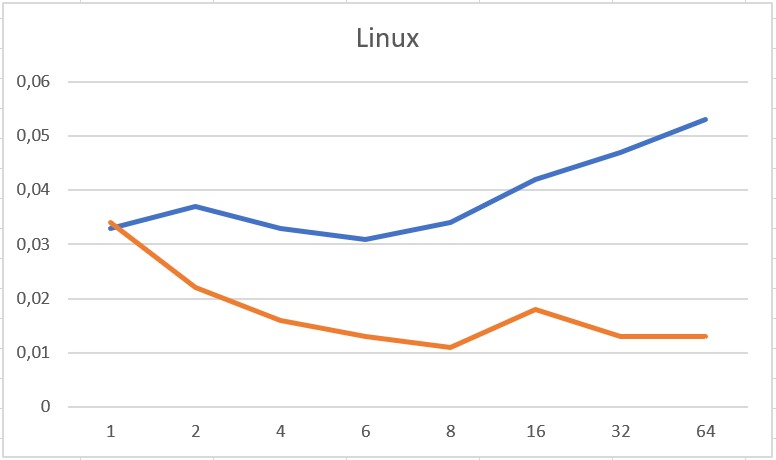
\includegraphics[scale=0.5]{linux.png}
\caption{Tiempos en Linux}
\end{figure}

\begin{figure}
\centering
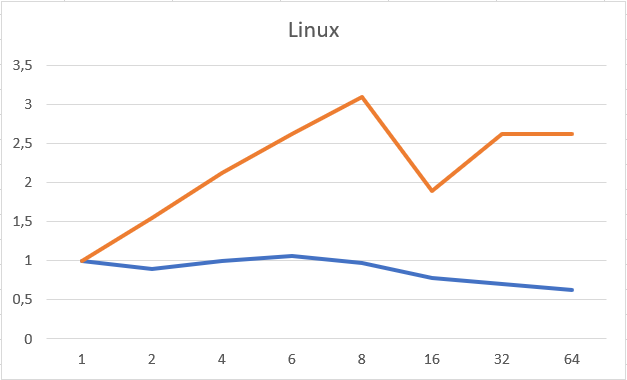
\includegraphics[scale=0.7]{speed-up linux.png}
\caption{SpeedUp en Linux}
\end{figure}


\end{document}




